\documentclass[11pt, oneside]{article}   	% use "amsart" instead of "article" for AMSLaTeX format
\usepackage{geometry}                		% See geometry.pdf to learn the layout options. There are lots.
\geometry{letterpaper}                   		% ... or a4paper or a5paper or ... 
%\geometry{landscape}                		% Activate for for rotated page geometry
%\usepackage[parfill]{parskip}    		% Activate to begin paragraphs with an empty line rather than an indent
\usepackage{graphicx}				% Use pdf, png, jpg, or eps� with pdflatex; use eps in DVI mode
								% TeX will automatically convert eps --> pdf in pdflatex		
\usepackage{amssymb}
\usepackage{amsmath}

\title{Fundamental Statistics}
%\author{The Author}
\date{}							% Activate to display a given date or no date

\graphicspath{{/Users/telliott_admin/Dropbox/Tex/png/}}
\begin{document}

\maketitle
%\section{}
% \subsection*{R code}
% \begin{lstlisting}  \end{lstlisting}
% \begin{center} 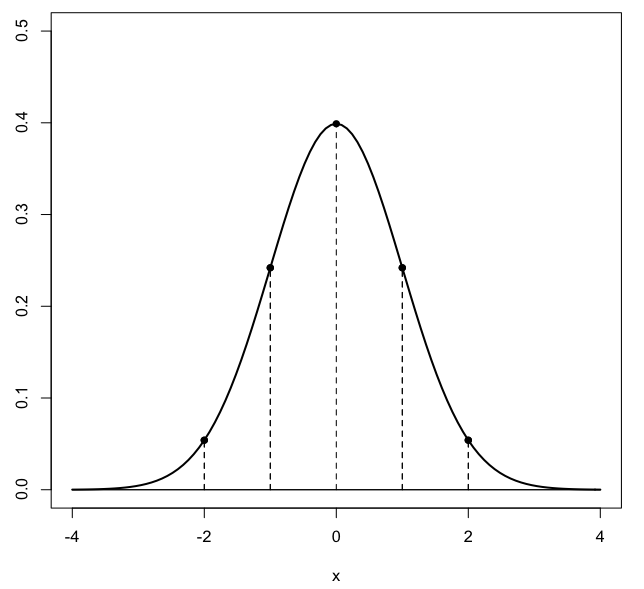
\includegraphics [scale=0.4] {gauss3.png} \end{center}
% \begin{bmatrix} a  &  b \\ c  &  d \end{bmatrix}
% \bigg |_

\large
\noindent Suppose we have a set of values $x_i$, which might be observations in a scientific experiment, or random samples from a larger population with some unknown distribution.  The standard measure of central tendency is the mean, $\mu$
\[ \mu_x = \frac{\sum x_i}{N} \]
where $N$ is the number of values in the sample. For example
\[ X = [1,2,3,4,5] \]
\[ \mu_X = \bar{X} = (1 + 2 + 3 + 4 + 5)/5 = 15/5 = 3 \]

An alternative measure is the median, which is at the halfway point.  If the values are ordered from largest to smallest and N is odd, then the median value is that value with $(N-1)/2$ values both above and below it in the list.  
\[ X = [1,2,3,4,5] \]
\[ med(X) = 3 \]
If N is even, then the two values which straddle the median are averaged and that is the value reported.  The mean is seen more often, but the median is particularly useful because it is not skewed by outliers.  (Bill Gates walks into a bar.  Suddenly the mean net worth of the customers is one billion dollars).
\[ X = [1,2,3,4] \]
\[ med(X) = (2+3)/2 = 2.5 \]

The variance of a set of values is written V or var
\[ var = \frac{1}{N} \sum (x_i - \mu_x)^2 \]
For some purposes (when we want the sample mean for draws from some larger population), the factor in front is $1/(N-1)$.

Standard deviation is the square root of the variance.
\[ \sigma = \sqrt{V} = \sqrt{\frac{1}{N} \sum (x_i - \mu_x)^2} \]
\subsection*{paired values}

Now suppose that in addition to $X = {x_1, x_2 \cdots x_N}$, we have $Y = {y_1, y_2 \cdots y_N}$---pairs of values.

Covariance is defined to be
\[ cov = \frac{1}{N} \sum (x_i - \mu_x)\sum (y_i - \mu_y) \]
Suppose 
\[ X = [1,2,3,4,5] \]
\[ Y = [10,8,6,4,2] \]
\[ cov(X,Y) = \frac{1}{N}((2)(4) + (1)(2) + (0)(0) + (1)(-2) + (2)(-4)) \]
One way to remember this is that
\[ cov(X,X) = Var(X,X) \]



\end{document}  